\documentclass[a5paper,11pt]{article}


%for coloring cell in a table
\usepackage[table]{xcolor}% http://ctan.org/pkg/xcolor

\usepackage{amsmath}
\usepackage{amssymb}

% for proofs  environment
\usepackage{amsthm}

% for 3d plots
\usepackage{pgfplots}
\usepackage{pgfplotstable}
\usepgfplotslibrary{patchplots}

\usepackage[backend=bibtex]{biblatex}
\bibliography{studio5}

% for probability trees
\usepackage{tikz}
\usetikzlibrary{trees}

% for Venn diagrams
\usetikzlibrary{shapes,backgrounds}

% for plots
\usepackage{ pgfplots}
% inserted on suggestion in warning during compilation
\pgfplotsset{compat=1.9}

%for strikethrough text
\usepackage{soul}

%for R source code listing
\usepackage{listings}

%for block quotes
\usepackage{csquotes}

\newtheorem{thm}{Theorem}
\newtheorem{lem}[thm]{Lemma}

% For not indenting the first line of paragraphs:
\setlength{\parindent}{0pt}
% define the title
\author{John Hancock}
\title{Studio 5}
\begin{document}
% generates the title
\maketitle
% insert the table of contents
\tableofcontents
\section{References and License}
We are answering questions in the material from MIT OpenCourseWare
course 18.05, Introduction to Probability and Statistics.

In this document we are answering questions Orloff and Bloom ask in
\cite{studio5}.

Please see the references section for detailed citation information.

The material for the course is licensed under the terms at
\url{http://ocw.mit.edu/terms}.

We use documentation in to write the \LaTeX source code for this document.

\section{Compare posterior distributions}

Orloff and Bloom ask us to change the prior probability distribution from
a uniformly distributed probability of $0.2$ for each type of dice to
a probability of $0.05$ for each type of
dice, except the $20$-sided die.  We assign a $0.8$ probability for
selecting the $20$-sided die.

This table shows the posterior distribution with uniformly distributed
probability of selecting any kind of die:

\begin{lstlisting}
[1] "Bayes table after one roll 1 : roll = 3"
  dice prior likelihood posterior.prenormalize posterior.normalized
1    4   0.2 0.25000000             0.05000000           0.37037037
2    6   0.2 0.16666667             0.03333333           0.24691358
3    8   0.2 0.12500000             0.02500000           0.18518519
4   12   0.2 0.08333333             0.01666667           0.12345679
5   20   0.2 0.05000000             0.01000000           0.07407407
\end{lstlisting}

This table show the posterior distribution where we alter the
prior distrubtion so that it is far more probable that we select
the 20-sided die:

\begin{lstlisting}
[1] "Bayes table after one roll 1 : roll = 8"
  dice prior likelihood posterior.prenormalize posterior.normalized
1    4  0.05 0.00000000            0.000000000           0.00000000
2    6  0.05 0.00000000            0.000000000           0.00000000
3    8  0.05 0.12500000            0.006250000           0.12396694
4   12  0.05 0.08333333            0.004166667           0.08264463
5   20  0.80 0.05000000            0.040000000           0.79338843
\end{lstlisting}

We see that the posterior distribution changes to reflect the increased
probabiliy of selecting the 20 sided die.

The stacked bar charts below show how the posteriror distributions change
as we update as we obtain more data from rolling the die.

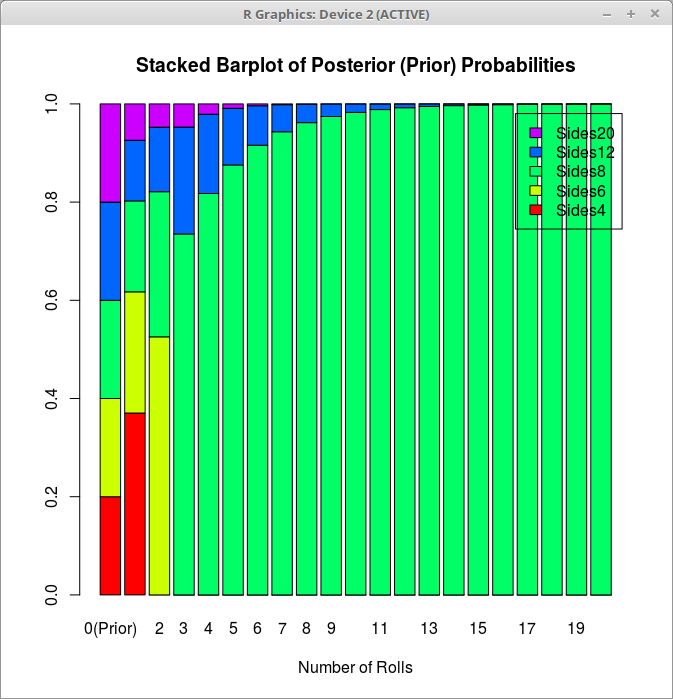
\includegraphics[scale=0.5]{uniform-dist.png}
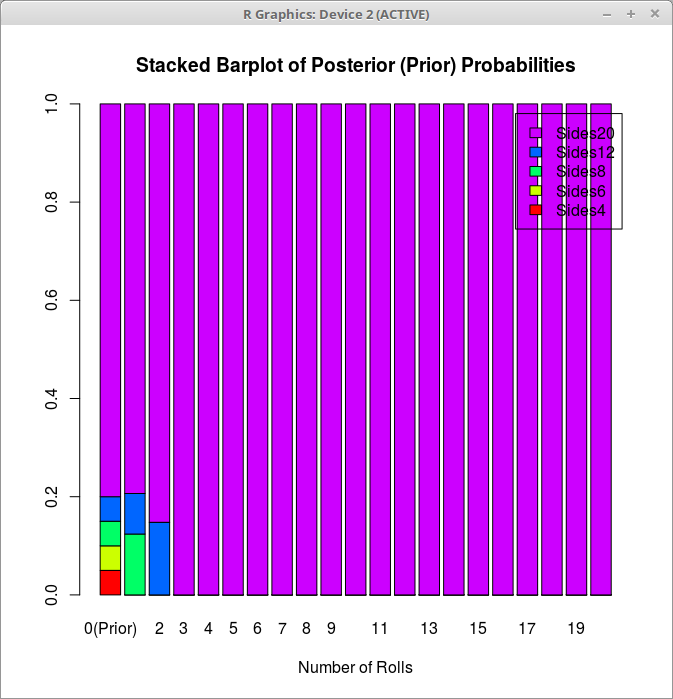
\includegraphics[scale=0.5]{skewed-dist.png}

\section{Uniform distribution, force $20$-sided die}
Orloff and Bloom ask us to run the simulation where we set the die that
the software selects to be the $20$-sided die.

The image below shows how the updating changes when we assume there is a
$20\%$ chance of selecting any die, and update probabilities as we obtain
more data.

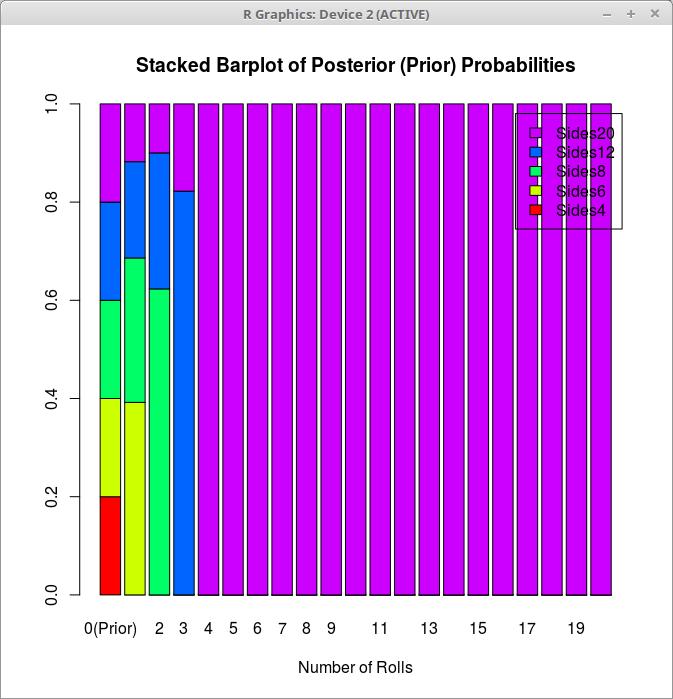
\includegraphics[scale=0.5]{force-20.png}

We see that the updating takes a bit longer to converge on the high probability
that we are seeing data from rolling a $20$-sided die.

\section{Censored data}
In this section, Orloff and Bloom ask us to consider censoring the data 
such that we record a zero if we roll anything other than a one.  If
we roll a one with any of the dice, we record a one.

\subsection{All possible hypotheses}
The possible hypothesis do not change; therefore the hypotheses are:
\begin{itemize}
\item $\mathcal{H}_4$ the die has four sides
\item $\mathcal{H}_6$ the die has six sides
\item $\mathcal{H}_8$ the die has eight sides
\item $\mathcal{H}_{12}$ the die has twelve sides
\item $\mathcal{H}_{20}$ the die has twenty sides
\end{itemize}

\subsection{Likelihood table}
Here is the likelihood table for one roll, $y_j$:

\begin{center}
\begin{tabular}{ | c | c | c | }
    \hline
    Hypothesis          & $y_j = 0$       & $y_j = 1$     \\ \hline
    $\mathcal{H}_{4}$   & $\frac{3}{4}$   & $\frac{1}{4}$ \\ \hline
    $\mathcal{H}_{6}$   & $\frac{5}{6}$   & $\frac{1}{6}$ \\ \hline
    $\mathcal{H}_{8}$   & $\frac{7}{8}$   & $\frac{1}{8}$ \\ \hline
    $\mathcal{H}_{12}$  & $\frac{11}{12}$ & $\frac{1}{12}$ \\ \hline
    $\mathcal{H}_{20}$  & $\frac{19}{20}$   & $\frac{1}{20}$ \\ \hline

  \end{tabular}
\end{center}


\printbibliography{}

\end{document}
